\subsection{Curvas de compresión/expansión isotrópica de las estructuras 
cristalinas de entrenamiento}

La Figura \ref{fig:compresion} muestra las energías de DFT para las 108 
estructuras en el conjunto de entrenamiento, junto con las predicciones de
DFTB correspondientes a los conjuntos de parámetros A y B. En general, se 
encuentra un buen acuerdo para ambos conjuntos, aunque se aprecían diferencias
mayores en las curvas de compresión para los elementos puros con el conjunto 
A de parámetros. Esto es consistente con el peso relativo bajo que se obtuvo
para los mismos en el proceso de ajuste (ver Tabla \ref{t:xiweights}). Por lo 
tanto, está variación mayor en la energía para los elementos puros es una 
consecuencia del algoritmo de optimización de pesos. Sin embargo, cabe 
destacar de nuevo que el objetivo es obtener una transferibilidad de los 
parámetros sobre un intervalo amplio de fracciones molares al centrar el 
modelo en reproducir las energías relativas en vez de sus valores absolutos.

\begin{figure}[th]
    \centering
    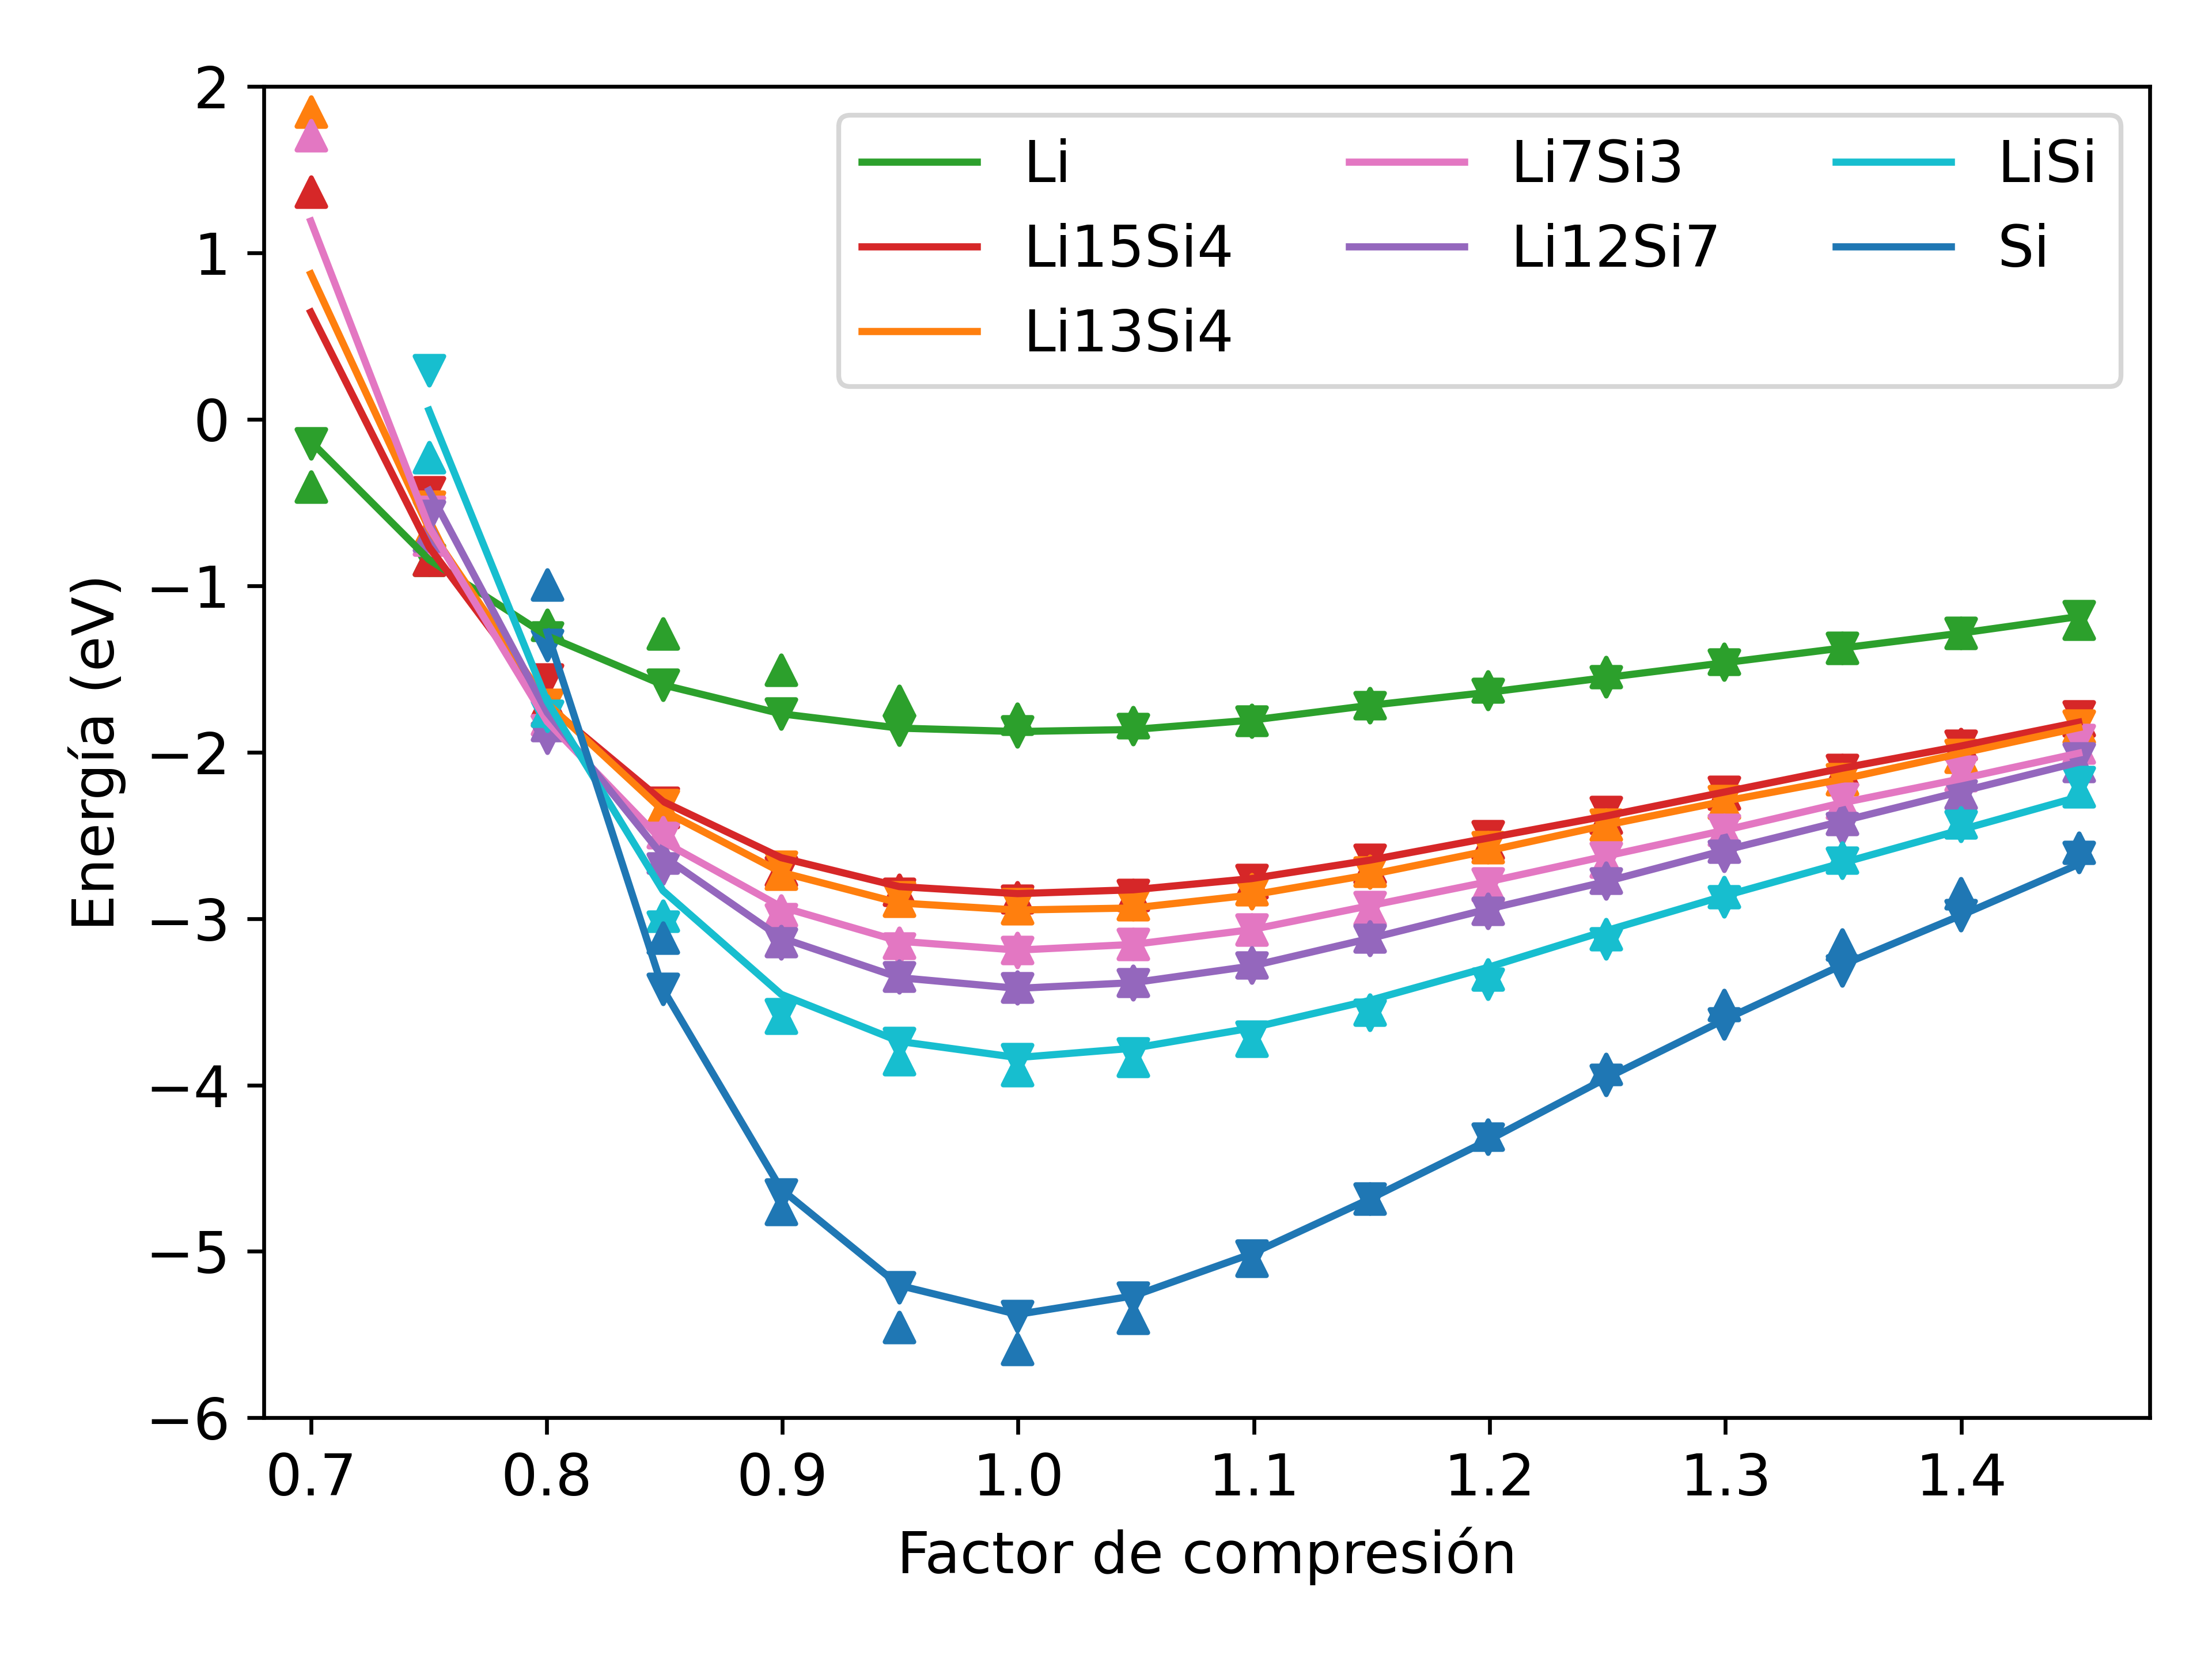
\includegraphics[width=.7\textwidth]{Silicio/modelo/resultados/compresion/compresion.png}
    \caption{Perfiles de energía para la compresión/expansión isotrópica de las 
    estructuras cristalinas de Li-Si, calculadas usando DFT (líneas continuas) 
    y DFTB con los conjuntos A (triángulos apuntando hacia arriba) y B 
    (triángulos apuntando hacia abajo) de parámetros.}
    \label{fig:compresion}
\end{figure}
